\chapter{Das Neuron}

\section{Struktur einer Nervenzelle}

\begin{figure}[h]
	\centering
		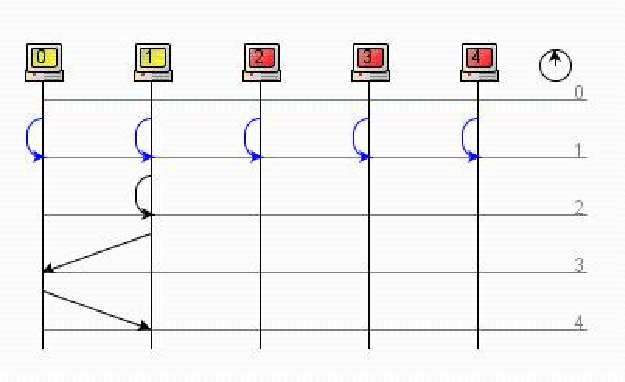
\includegraphics{images/p1ReadSeq.pdf}
\caption{Aufbau einer Nervenzelle}
\small
 1. Dendrite\footnotemark[1] leiten 
 afferente\footnotemark[2] Signale zum 
 2. Soma\footnotemark[3], dem Zellkörper, weiter. 
 3. Axon\footnotemark[4] leitet ein 
 efferentes\footnotemark[5] Nervensignal über präsynaptische Endigungen (Axonterminale) an (häufig weit 
 entfernte\footnotemark[6]) 
 Effektoren\footnotemark[7]
 wie Muskeln und Drüsen oder nachgeschaltete Neuronen 
 weiter\footnotemark[8] {[SD07, S. 42, Abs. 2]}

\end{figure}

\footnotetext[1]{``\textgreek{δένδρον} (dendrón)`` (altgriechisch): Baum}
\footnotetext[2]{``afferre`` (lat.): herbeibringen, melden, bringen}
\footnotetext[3]{``\textgreek{σῶμα} (sõma)`` (altgriechisch): Körper}
\footnotetext[4]{``axon`` (lat.): Achse}
\footnotetext[5]{``efferre`` (lat.): hinaustragen, mitnehmen}
\footnotetext[6]{Axone können sich im menschlichen Körper über Entfernungen von bis zu über 1m ausstrecken {[BCP18, S. 28, Abs. 2]}}
\footnotetext[7]{``efficere`` (lat.): bewirken, hervorbringen} 
\footnotetext[8]{in diesem Fall empfangen postsynaptische Rezeptoren an den Dendriten des nachgeschalteten Neurons ein Signal und der beschriebene Prozess wiederholt sich. Bildlich können wir uns Effektoren als Endglied der Signalübertragung vorstellen, auch wenn hier wieder interzelluläre Vorgänge stattfinden. Vgl. ``neuromuskuläre Endplatte`` {[BCP18, S. 127, Abs. 3]}} 

Die eingehende Schnittstelle eines Neurons sind seine \textbf{Dendriten}: Baumförmige Fortsätze\footnotemark[9], die um das \textbf{Soma} herum gelagert sind. Diese Dendritenbäume [BCP18:47] fungieren \textit{postsynaptisch} und empfangen afferente Signale in Form von Neurotransmittern [Eil19:61, ``Synapsen``]. Diese werden von Rezeptoren, die sich an den Enden der Dendriten befinden, aufgenommen. Oft stehen tausende Neuronen in Verbindung mit den Dendriten eines einzelnen Neurons\footnotemark[10] [SD07, S .42].\\


Die \textbf{Dendriten} leiten Signale weiter an das Soma (oder \textit{Perikaryon} [RK18:58, ``Aufbau``], den Zellkörper und das Stoffwechselzentrum des Neurons, der eine Größe von ca. 20 μm\footnotemark[11] [BCP18:29] besitzt. In der Zelle befindet sich - durch die \textit{Neuronenmembran}\footnotemark[12] von der Umgebung getrennt - \textit{Zytosol}, eine salzige, wässrige Flüssigkeit mit einem hohen Anteil von Kalium [BCP18:29, ``Das Soma``]\footnotemark[13]. In dem Zytosol eingebettet sind weitere subzelluläre Strukturen mit eigener Membranbegrenzung, die \textit{Zellorganellen} [SD07:8, Abs. 2]. Für die nachfolgenden Untersuchungen interessieren uns bei dem Zellkörper aber vor allem die Zellmembran und der \textit{transmembranale Transport} von Ionen\footnotemark[14] zur Änderung des Membranpotenzials, insbesondere in der Nähe des \textbf{Axonhügels} (ca. 20-50 µm vom Soma [BLS19:77, ``Ort der Aktionspotenzialinitiation``]): Dort entspringt das \textbf{Axon}, welches in einer ``salzigen extrazellulären Flüssigkeit mit hoher Leitfähigkeit`` [PCB18:61, Abs. 1]\footnotemark[15] liegt. Hier entscheidet sich, ob das Neuron Informationen weiterleitet: Die Summation der durch die postsynaptischen Endigungen einhergehenden Signale kann eine Depolarisation\footnotemark[16] der Membran an dieser Stelle [Eil19, S. 61, ``Soma``] über einen gewissen \textbf{Schwellenwert} bewirken, so das ein \textbf{Aktionspotenzial} ausgelöst wird [BCP18, p.142 f.]. Dadurch wird in den präsynaptischen Endigungen die Exozytose ausgelöst.

\footnotetext[9]{einzelne selten länger als 2mm {[BCP18:28, Abs. 2]}. Längere Dendriten finden sich an den kortikalen Pyramidenzellen mit einer Länge von 1 cm {[Eil19:58, ``Polarisierung``]} }

\footnotetext[10]{das menschliche Gehirn besitzt mindestens $10^{11}$ Neuronen [KSJ+13:175, Abs. 2]}
\footnotetext[11]{ein menschliches Haar hat einen Durchmesser von ca. 70 μm, kleine Bakterien bis zu 20 μm}
\footnotetext[12]{Membrandicke ca. 5 nm {[BLS19:66, letzter Absatz linke Spalte]}}
\footnotetext[13]{ vgl. Ionenkonzentrationen in \textbf{Tab. 1.1}}
\footnotetext[14]{hier: der Austausch von Ionen zwischen dem intra- und extrazellulären Raum durch Kanäle und Pumpen. Zur Erinnerung: Ion bezeichnet ein elektrisch geladenes Atom oder Molekül.}
\footnotetext[15]{{[BCP18:43, Abs. 1]}, führt das Axon metaphorisch mit einer Telefonleitung zusammen. Aufgrund der signalempfangenden Eigenschaften und der dünnen Spitzen der Dendriten liegt auch der Vergleich mit ``Antennen`` nahe {[BCP18:28, Abs. 2]}}
\footnotetext[16]{\textit{Depolarisation} bezeichnet die Verringerung des Membranpotenzials von einem negativen Wert auf einen weniger negativen oder gar einen positiven Wert {[RHN+16:812 ``Neurotransmitter und ihre Rezeptoren``]}}

